%%%%%%%%%%%%%%%%%%%%%%%%%%%%%%%%%%%%%%%%%
%  My documentation report
%  Objetive: Explain what I did and how, so someone can continue with the investigation
%
% Important note:
% Chapter heading images should have a 2:1 width:height ratio,
% e.g. 920px width and 460px height.
%
%%%%%%%%%%%%%%%%%%%%%%%%%%%%%%%%%%%%%%%%%


%----------------------------------------------------------------------------------------
%	PACKAGES AND OTHER DOCUMENT CONFIGURATIONS
%----------------------------------------------------------------------------------------

\documentclass[11pt,fleqn]{book} % Default font size and left-justified equations

\usepackage[top=3cm,bottom=3cm,left=3.2cm,right=3.2cm,headsep=10pt,letterpaper]{geometry} % Page margins

\usepackage{xcolor} % Required for specifying colors by name
\definecolor{ocre}{RGB}{52,177,201} % Define the orange color used for highlighting throughout the book

% Font Settings
\usepackage{avant} % Use the Avantgarde font for headings
%\usepackage{times} % Use the Times font for headings
\usepackage{mathptmx} % Use the Adobe Times Roman as the default text font together with math symbols from the Sym­bol, Chancery and Com­puter Modern fonts
\usepackage{microtype} % Slightly tweak font spacing for aesthetics
\usepackage[utf8]{inputenc} % Required for including letters with accents
\usepackage[T1]{fontenc} % Use 8-bit encoding that has 256 glyphs
\usepackage{amsthm}

% Bibliography
\usepackage[style=alphabetic,sorting=nyt,sortcites=true,autopunct=true,babel=hyphen,hyperref=true,abbreviate=false,backref=true,backend=biber]{biblatex}
\addbibresource{bibliography.bib} % BibTeX bibliography file
\defbibheading{bibempty}{}

%----------------------------------------------------------------------------------------
%	VARIOUS REQUIRED PACKAGES
%----------------------------------------------------------------------------------------

\usepackage{titlesec} % Allows customization of titles

\usepackage{graphicx} % Required for including pictures
\graphicspath{{Pictures/}} % Specifies the directory where pictures are stored
% \graphicspath{{Plots/}}
\usepackage{lipsum} % Inserts dummy text

\usepackage{tikz} % Required for drawing custom shapes

\usepackage[english]{babel} % English language/hyphenation

\usepackage{enumitem} % Customize lists
\setlist{nolistsep} % Reduce spacing between bullet points and numbered lists

\usepackage{booktabs} % Required for nicer horizontal rules in tables

\usepackage{eso-pic} % Required for specifying an image background in the title page

%----------------------------------------------------------------------------------------
%	MAIN TABLE OF CONTENTS
%----------------------------------------------------------------------------------------

\usepackage{titletoc} % Required for manipulating the table of contents

\contentsmargin{0cm} % Removes the default margin
% Chapter text styling
\titlecontents{chapter}[1.25cm] % Indentation
{\addvspace{15pt}\large\sffamily\bfseries} % Spacing and font options for chapters
{\color{ocre!60}\contentslabel[\Large\thecontentslabel]{1.25cm}\color{ocre}} % Chapter number
{}  
{\color{ocre!60}\normalsize\sffamily\bfseries\;\titlerule*[.5pc]{.}\;\thecontentspage} % Page number
% Section text styling
\titlecontents{section}[1.25cm] % Indentation
{\addvspace{5pt}\sffamily\bfseries} % Spacing and font options for sections
{\contentslabel[\thecontentslabel]{1.25cm}} % Section number
{}
{\sffamily\hfill\color{black}\thecontentspage} % Page number
[]
% Subsection text styling
\titlecontents{subsection}[1.25cm] % Indentation
{\addvspace{1pt}\sffamily\small} % Spacing and font options for subsections
{\contentslabel[\thecontentslabel]{1.25cm}} % Subsection number
{}
{\sffamily\;\titlerule*[.5pc]{.}\;\thecontentspage} % Page number
[] 

%----------------------------------------------------------------------------------------
%	MINI TABLE OF CONTENTS IN CHAPTER HEADS
%----------------------------------------------------------------------------------------

% Section text styling
\titlecontents{lsection}[0em] % Indendating
{\footnotesize\sffamily} % Font settings
{}
{}
{}

% Subsection text styling
\titlecontents{lsubsection}[.5em] % Indentation
{\normalfont\footnotesize\sffamily} % Font settings
{}
{}
{}
 
%----------------------------------------------------------------------------------------
%	PAGE HEADERS
%----------------------------------------------------------------------------------------

\usepackage{fancyhdr} % Required for header and footer configuration

\pagestyle{fancy}
\renewcommand{\chaptermark}[1]{\markboth{\sffamily\normalsize\bfseries\chaptername\ \thechapter.\ #1}{}} % Chapter text font settings
\renewcommand{\sectionmark}[1]{\markright{\sffamily\normalsize\thesection\hspace{5pt}#1}{}} % Section text font settings
\fancyhf{} \fancyhead[LE,RO]{\sffamily\normalsize\thepage} % Font setting for the page number in the header
\fancyhead[LO]{\rightmark} % Print the nearest section name on the left side of odd pages
\fancyhead[RE]{\leftmark} % Print the current chapter name on the right side of even pages
\renewcommand{\headrulewidth}{0.5pt} % Width of the rule under the header
\addtolength{\headheight}{2.5pt} % Increase the spacing around the header slightly
\renewcommand{\footrulewidth}{0pt} % Removes the rule in the footer
\fancypagestyle{plain}{\fancyhead{}\renewcommand{\headrulewidth}{0pt}} % Style for when a plain pagestyle is specified

% Removes the header from odd empty pages at the end of chapters
\makeatletter
\renewcommand{\cleardoublepage}{
\clearpage\ifodd\c@page\else
\hbox{}
\vspace*{\fill}
\thispagestyle{empty}
\newpage
\fi}

%----------------------------------------------------------------------------------------
%	THEOREM STYLES
%----------------------------------------------------------------------------------------

\usepackage{amsmath,amsfonts,amssymb,amsthm} % For math equations, theorems, symbols, etc

\newcommand{\intoo}[2]{\mathopen{]}#1\,;#2\mathclose{[}}
\newcommand{\ud}{\mathop{\mathrm{{}d}}\mathopen{}}
\newcommand{\intff}[2]{\mathopen{[}#1\,;#2\mathclose{]}}
\newtheorem{notation}{Notation}[chapter]

%%%%%%%%%%%%%%%%%%%%%%%%%%%%%%%%%%%%%%%%%%%%%%%%%%%%%%%%%%%%%%%%%%%%%%%%%%%
%%%%%%%%%%%%%%%%%%%% dedicated to boxed/framed environements %%%%%%%%%%%%%%
%%%%%%%%%%%%%%%%%%%%%%%%%%%%%%%%%%%%%%%%%%%%%%%%%%%%%%%%%%%%%%%%%%%%%%%%%%%
\newtheoremstyle{ocrenumbox}% % Theorem style name
{0pt}% Space above
{0pt}% Space below
{\normalfont}% % Body font
{}% Indent amount
{\small\bf\sffamily\color{ocre}}% % Theorem head font
{\;}% Punctuation after theorem head
{0.25em}% Space after theorem head
{\small\sffamily\color{ocre}\thmname{#1}\nobreakspace\thmnumber{\@ifnotempty{#1}{}\@upn{#2}}% Theorem text (e.g. Theorem 2.1)
\thmnote{\nobreakspace\the\thm@notefont\sffamily\bfseries\color{black}---\nobreakspace#3.}} % Optional theorem note
\renewcommand{\qedsymbol}{$\blacksquare$}% Optional qed square

\newtheoremstyle{blacknumex}% Theorem style name
{5pt}% Space above
{5pt}% Space below
{\normalfont}% Body font
{} % Indent amount
{\small\bf\sffamily}% Theorem head font
{\;}% Punctuation after theorem head
{0.25em}% Space after theorem head
{\small\sffamily{\tiny\ensuremath{\blacksquare}}\nobreakspace\thmname{#1}\nobreakspace\thmnumber{\@ifnotempty{#1}{}\@upn{#2}}% Theorem text (e.g. Theorem 2.1)
\thmnote{\nobreakspace\the\thm@notefont\sffamily\bfseries---\nobreakspace#3.}}% Optional theorem note

\newtheoremstyle{blacknumbox} % Theorem style name
{0pt}% Space above
{0pt}% Space below
{\normalfont}% Body font
{}% Indent amount
{\small\bf\sffamily}% Theorem head font
{\;}% Punctuation after theorem head
{0.25em}% Space after theorem head
{\small\sffamily\thmname{#1}\nobreakspace\thmnumber{\@ifnotempty{#1}{}\@upn{#2}}% Theorem text (e.g. Theorem 2.1)
\thmnote{\nobreakspace\the\thm@notefont\sffamily\bfseries---\nobreakspace#3.}}% Optional theorem note

%%%%%%%%%%%%%%%%%%%%%%%%%%%%%%%%%%%%%%%%%%%%%%%%%%%%%%%%%%%%%%%%%%%%%%%%%%%
%%%%%%%%%%%%% dedicated to non-boxed/non-framed environements %%%%%%%%%%%%%
%%%%%%%%%%%%%%%%%%%%%%%%%%%%%%%%%%%%%%%%%%%%%%%%%%%%%%%%%%%%%%%%%%%%%%%%%%%
\newtheoremstyle{ocrenum}% % Theorem style name
{5pt}% Space above
{5pt}% Space below
{\normalfont}% % Body font
{}% Indent amount
{\small\bf\sffamily\color{ocre}}% % Theorem head font
{\;}% Punctuation after theorem head
{0.25em}% Space after theorem head
{\small\sffamily\color{ocre}\thmname{#1}\nobreakspace\thmnumber{\@ifnotempty{#1}{}\@upn{#2}}% Theorem text (e.g. Theorem 2.1)
\thmnote{\nobreakspace\the\thm@notefont\sffamily\bfseries\color{black}---\nobreakspace#3.}} % Optional theorem note
\renewcommand{\qedsymbol}{$\blacksquare$}% Optional qed square
\makeatother

% Defines the theorem text style for each type of theorem to one of the three styles above
\newcounter{dummy} 
\numberwithin{dummy}{section}
\theoremstyle{ocrenumbox}


\newtheorem{theoremeT}[dummy]{Theorem}
\newtheorem{lemma}[dummy]{Lemma}
\newtheorem{observation}[dummy]{Observation}
\newtheorem{proposition}[dummy]{Proposition}
% \newtheorem{definition}[dummy]{Definition}
\newtheorem{claim}[dummy]{Claim}
\newtheorem{fact}[dummy]{Fact}
\newtheorem{assumption}[dummy]{Assumption}

\newtheorem{problem}{Problem}[chapter]
% \newtheorem{exercise}{Exercise}[chapter]
\theoremstyle{blacknumex}
\newtheorem{exampleT}{Example}[chapter]
\theoremstyle{blacknumbox}
\newtheorem{vocabulary}{Vocabulary}[chapter]
\newtheorem{definitionT}{Definition}[section]
\newtheorem{corollaryT}[dummy]{Corollary}
\theoremstyle{ocrenum}

%----------------------------------------------------------------------------------------
%	DEFINITION OF COLORED BOXES
%----------------------------------------------------------------------------------------

\RequirePackage[framemethod=default]{mdframed} % Required for creating the theorem, definition, exercise and corollary boxes

% Theorem box
\newmdenv[skipabove=7pt,
skipbelow=7pt,
backgroundcolor=black!5,
linecolor=ocre,
innerleftmargin=5pt,
innerrightmargin=5pt,
innertopmargin=5pt,
leftmargin=0cm,
rightmargin=0cm,
innerbottommargin=5pt]{tBox}

% Exercise box	  
\newmdenv[skipabove=7pt,
skipbelow=7pt,
rightline=false,
leftline=true,
topline=false,
bottomline=false,
backgroundcolor=ocre!10,
linecolor=ocre,
innerleftmargin=5pt,
innerrightmargin=5pt,
innertopmargin=5pt,
innerbottommargin=5pt,
leftmargin=0cm,
rightmargin=0cm,
linewidth=4pt]{eBox}	

% Definition box
\newmdenv[skipabove=7pt,
skipbelow=7pt,
rightline=false,
leftline=true,
topline=false,
bottomline=false,
linecolor=ocre,
innerleftmargin=5pt,
innerrightmargin=5pt,
innertopmargin=0pt,
leftmargin=0cm,
rightmargin=0cm,
linewidth=4pt,
innerbottommargin=0pt]{dBox}	

% Corollary box
\newmdenv[skipabove=7pt,
skipbelow=7pt,
rightline=false,
leftline=true,
topline=false,
bottomline=false,
linecolor=gray,
backgroundcolor=black!5,
innerleftmargin=5pt,
innerrightmargin=5pt,
innertopmargin=5pt,
leftmargin=0cm,
rightmargin=0cm,
linewidth=4pt,
innerbottommargin=5pt]{cBox}

% Creates an environment for each type of theorem and assigns it a theorem text style from the "Theorem Styles" section above and a colored box from above
\newenvironment{theorem}{\begin{tBox}\begin{theoremeT}}{\end{theoremeT}\end{tBox}}
\newenvironment{exercise}{\begin{eBox}\begin{exerciseT}}{\hfill{\color{ocre}\tiny\ensuremath{\blacksquare}}\end{exerciseT}\end{eBox}}				  
\newenvironment{definition}{\begin{dBox}\begin{definitionT}}{\end{definitionT}\end{dBox}}	
\newenvironment{example}{\begin{exampleT}}{\hfill{\tiny\ensuremath{\blacksquare}}\end{exampleT}}		
\newenvironment{corollary}{\begin{cBox}\begin{corollaryT}}{\end{corollaryT}\end{cBox}}	

%----------------------------------------------------------------------------------------
%	REMARK ENVIRONMENT
%----------------------------------------------------------------------------------------

\newenvironment{remark}{\par\vspace{10pt}\small % Vertical white space above the remark and smaller font size
\begin{list}{}{
\leftmargin=35pt % Indentation on the left
\rightmargin=25pt}\item\ignorespaces % Indentation on the right
\makebox[-2.5pt]{\begin{tikzpicture}[overlay]
\node[draw=ocre!60,line width=1pt,circle,fill=ocre!25,font=\sffamily\bfseries,inner sep=2pt,outer sep=0pt] at (-15pt,0pt){\textcolor{ocre}{R}};\end{tikzpicture}} % Orange R in a circle
\advance\baselineskip -1pt}{\end{list}\vskip5pt} % Tighter line spacing and white space after remark

%----------------------------------------------------------------------------------------
%	SECTION NUMBERING IN THE MARGIN
%----------------------------------------------------------------------------------------

\makeatletter
\renewcommand{\@seccntformat}[1]{\llap{\textcolor{ocre}{\csname the#1\endcsname}\hspace{1em}}}                    
\renewcommand{\section}{\@startsection{section}{1}{\z@}
{-4ex \@plus -1ex \@minus -.4ex}
{1ex \@plus.2ex }
{\normalfont\large\sffamily\bfseries}}
\renewcommand{\subsection}{\@startsection {subsection}{2}{\z@}
{-3ex \@plus -0.1ex \@minus -.4ex}
{0.5ex \@plus.2ex }
{\normalfont\sffamily\bfseries}}
\renewcommand{\subsubsection}{\@startsection {subsubsection}{3}{\z@}
{-2ex \@plus -0.1ex \@minus -.2ex}
{.2ex \@plus.2ex }
{\normalfont\small\sffamily\bfseries}}                        
\renewcommand\paragraph{\@startsection{paragraph}{4}{\z@}
{-2ex \@plus-.2ex \@minus .2ex}
{.1ex}
{\normalfont\small\sffamily\bfseries}}

%----------------------------------------------------------------------------------------
%	HYPERLINKS IN THE DOCUMENTS
%----------------------------------------------------------------------------------------

% For an unclear reason, the package should be loaded now and not later
\usepackage{hyperref}
\hypersetup{hidelinks,backref=true,pagebackref=true,hyperindex=true,colorlinks=false,breaklinks=true,urlcolor= ocre,bookmarks=true,bookmarksopen=false,pdftitle={Title},pdfauthor={Author}}

%----------------------------------------------------------------------------------------
%	CHAPTER HEADINGS
%----------------------------------------------------------------------------------------

% The set-up below should be (sadly) manually adapted to the overall margin page septup controlled by the geometry package loaded in the main.tex document. It is possible to implement below the dimensions used in the goemetry package (top,bottom,left,right)... TO BE DONE

\newcommand{\thechapterimage}{}
\newcommand{\chapterimage}[1]{\renewcommand{\thechapterimage}{#1}}

% Numbered chapters with mini tableofcontents
\def\thechapter{\arabic{chapter}}
\def\@makechapterhead#1{
\thispagestyle{empty}
{\centering \normalfont\sffamily
\ifnum \c@secnumdepth >\m@ne
\if@mainmatter
\startcontents
\begin{tikzpicture}[remember picture,overlay]
\node at (current page.north west)
{\begin{tikzpicture}[remember picture,overlay]
\node[anchor=north west,inner sep=0pt] at (0,0) {\includegraphics[width=\paperwidth]{\thechapterimage}};
%%%%%%%%%%%%%%%%%%%%%%%%%%%%%%%%%%%%%%%%%%%%%%%%%%%%%%%%%%%%%%%%%%%%%%%%%%%%%%%%%%%%%
% Commenting the 3 lines below removes the small contents box in the chapter heading
%\fill[color=ocre!10!white,opacity=.6] (1cm,0) rectangle (8cm,-7cm);
%\node[anchor=north west] at (1.1cm,.35cm) {\parbox[t][8cm][t]{6.5cm}{\huge\bfseries\flushleft \printcontents{l}{1}{\setcounter{tocdepth}{2}}}};
\draw[anchor=west] (5cm,-9cm) node [rounded corners=20pt,fill=ocre!10!white,text opacity=1,draw=ocre,draw opacity=1,line width=1.5pt,fill opacity=.6,inner sep=12pt]{\huge\sffamily\bfseries\textcolor{black}{\thechapter. #1\strut\makebox[22cm]{}}};
%%%%%%%%%%%%%%%%%%%%%%%%%%%%%%%%%%%%%%%%%%%%%%%%%%%%%%%%%%%%%%%%%%%%%%%%%%%%%%%%%%%%%
\end{tikzpicture}};
\end{tikzpicture}}
\par\vspace*{230\p@}
\fi
\fi}

% Unnumbered chapters without mini tableofcontents (could be added though) 
\def\@makeschapterhead#1{
\thispagestyle{empty}
{\centering \normalfont\sffamily
\ifnum \c@secnumdepth >\m@ne
\if@mainmatter
\begin{tikzpicture}[remember picture,overlay]
\node at (current page.north west)
{\begin{tikzpicture}[remember picture,overlay]
\node[anchor=north west,inner sep=0pt] at (0,0) {\includegraphics[width=\paperwidth]{\thechapterimage}};
\draw[anchor=west] (5cm,-9cm) node [rounded corners=20pt,fill=ocre!10!white,fill opacity=.6,inner sep=12pt,text opacity=1,draw=ocre,draw opacity=1,line width=1.5pt]{\huge\sffamily\bfseries\textcolor{black}{#1\strut\makebox[22cm]{}}};
\end{tikzpicture}};
\end{tikzpicture}}
\par\vspace*{230\p@}
\fi
\fi
}
\makeatother % Insert the commands.tex file which contains the majority of the structure behind the template

%----------------------------------------------------------------------------------------
%	Definitions of new commands
%----------------------------------------------------------------------------------------

\def\R{\mathbb{R}}
\newcommand{\cvx}{convex}
\begin{document}

%----------------------------------------------------------------------------------------
%	TITLE PAGE
%----------------------------------------------------------------------------------------

\begingroup
\thispagestyle{empty}
\AddToShipoutPicture*{\put(0,0){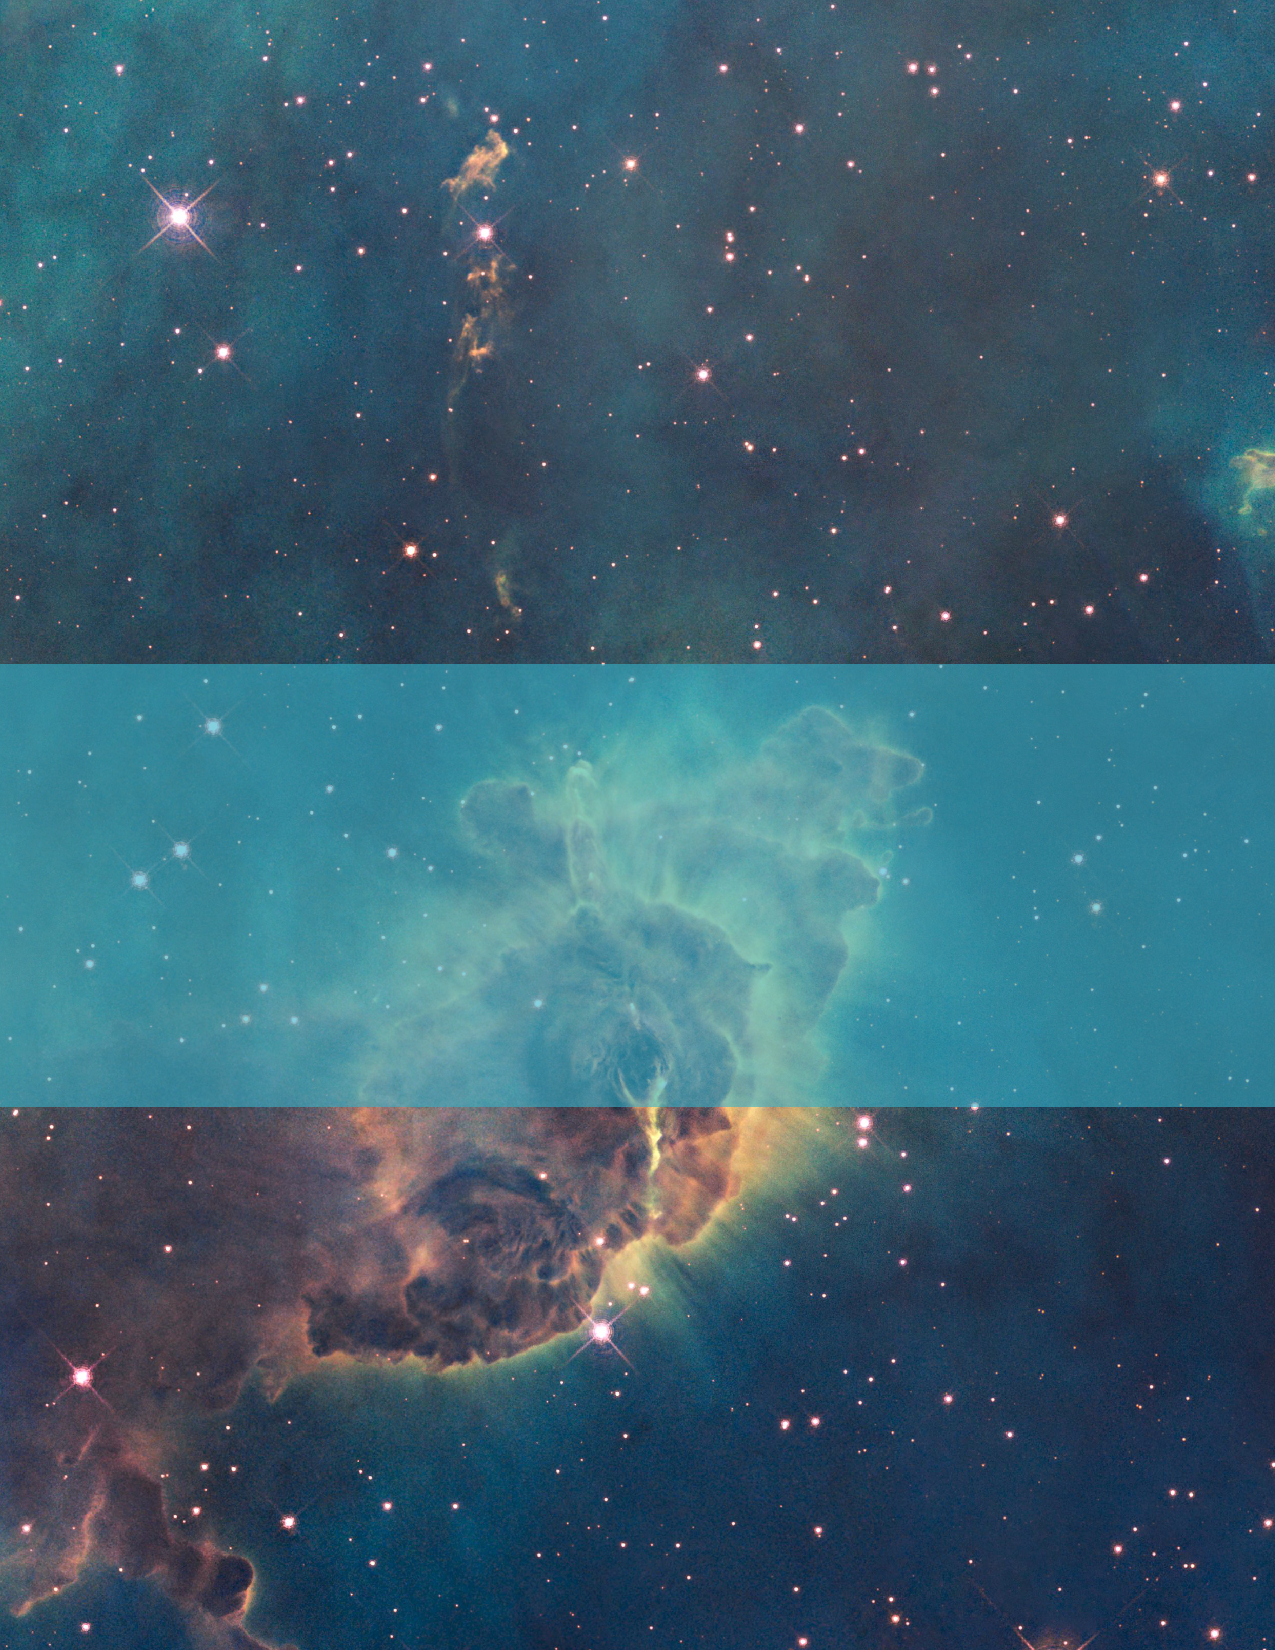
\includegraphics[scale=1.25]{esahubble}}} % Image background
\centering
\vspace*{5cm}
\par\normalfont\fontsize{35}{35}\sffamily\selectfont
\textbf{Computational Biology 2021}\\
{\LARGE Expectation-Maximization of the Potential of Mean Force}\par % Book title
\vspace*{1cm}
{\Huge Technical Report}\par % Author name
\endgroup

%----------------------------------------------------------------------------------------
%	COPYRIGHT PAGE
%----------------------------------------------------------------------------------------

\newpage
~\vfill
\thispagestyle{empty}

%\noindent Copyright \copyright\ 2014 Andrea Hidalgo\\ % Copyright notice

\noindent \textsc{Biosystems Simulation Lab, National Chiao Tung University}\\

\noindent \textsc{https://github.com/yizaochen/em_theory}\\ % URL

\noindent This research was done under the supervision of Dr. Jhih-Wei Chu with the financial support of MOST Taiwan.\\ % License information

\noindent \textit{First release, November 2020} % Printing/edition date

%----------------------------------------------------------------------------------------
%	TABLE OF CONTENTS
%----------------------------------------------------------------------------------------

\chapterimage{head1.png} % Table of contents heading image

\pagestyle{empty} % No headers

\tableofcontents % Print the table of contents itself

%\cleardoublepage % Forces the first chapter to start on an odd page so it's on the right

\pagestyle{fancy} % Print headers again

%----------------------------------------------------------------------------------------
%	CHAPTER 1
%----------------------------------------------------------------------------------------

\chapterimage{head2.png} % Chapter heading image
\chapter{Convex Sets}
\section{Convexity}
\subsection{Cone}
\begin{definition}[Cone]
A set $K \in \R^n$, when $x \in K $ implies $\alpha x \in K$.
\end{definition}
A non convex cone can be hyper-plane.\\
For convex cone $x + y \in K, \forall x,y \in K$.\\
Cone don't need to be "pointed". e.g. \\
Direct sums of cones $C_1 + C_2 = \{ x = x_1+x_2 | x_1 \in C_1, x_2 \in C_2 \}$.\\
\begin{example}
$S_1^n  \{ X | X=X^n ,\lambda(x) \ge 0\}$\\
A matrix with positive eigenvalues.
\end{example}

\subsubsection{Operations preserving convexity}
\begin{itemize}
\item[Intersection] $C  \cap_{i \in \mathbb{I}}C_i$
\item[Linear map] Let $A : \mathbb{R}^n \to  \R^n$ be a linear map. If $C \in \R^n$ is convex, so is $A(C) = \{Ax \forall x \in C \}$
\item[Inverse image] $A^{-1}(D) = \{ x \in \R |Ax \in D \}$
\end{itemize}

\subsubsection{Operations that induce convexity}
Convex hull on $S = \cap \{C | S\in C, C is convex\}$\\
\begin{example}
$Co \{ x_1,x_2,\cdots,x_m\} = \{ \sum_{i=1}^m \alpha_i x_i | \alpha \in \delta_m \}$
\end{example}
For a convex set $x \in C \Rightarrow x = \sum \alpha_i x_i$. 
\begin{theorem}[Carathéodory's theorem]
If a point $x \in \R^d$ lies in the convex hull of a set $P$, there is a subset $P'$ of $P$ consisting of $d + 1$ or fewer points such that $x$ lies in the convex hull of $P'$. Equivalently, x lies in an r-simplex with vertices in P.
\end{theorem}

\section{Convex Functions}
\begin{definition}[Convex function]
Let $C \in \R^n$ be convex, $f:C \to \R$ is convex on f if $x,y \in C \times C$. $\forall \alpha \in (0,1)$, $f(\alpha x + (1-\alpha) y) \le f(\alpha x) + f((1-\alpha) y)$
\end{definition}

\begin{definition}[Strictly Convex function]
Let $C \in \R^n$ be convex, $f:C \to \R$ is strictly convex on f if $x,y \in C \times C$. $\forall \alpha \in (0,1)$, $f(\alpha x + (1-\alpha) y) \langle f(\alpha x) + f((1-\alpha) y)$
\end{definition}

\begin{definition}[Strongly convex]
$f:C \to \R$ is strongly convex with modules $u \ge 0$ if $f - \frac{1}{2}u || \cdot ||^2$ is convex.
\end{definition}
Interpretation: There is a convex quadratic $\frac{1}{2}u || \cdot ||^2$ that lower bounds f.
\begin{example}
$\min_{x \in C} f(x) \leftrightarrow \min \bar{f}(x)$
Useful to turn this into an unconstrained problem. \\
$$\bar{f}(x) = \begin{cases}
f(x) \quad if x \in C \\
\infty \quad  elsewhere
\end{cases}$$
\end{example}
\begin{definition}
A function $f : \R^n \to \R \cup \infty \ \bar{\R}$ is convex if $x,y \in \R^n \times \R^n$, $\forall x,y , \bar{f}(\alpha x + (1-\alpha) y) \le f(\alpha x) + f((1-\alpha) y)$
\end{definition}
Definition 1 is equivalent to definition 2 if $f(x) = \infty$.
\begin{example}
$f(x) = \sup_{j \in J} f_j(x)$
\end{example}

\subsection{Epigraph} 
\begin{definition}[Epigraph]
For $f: \R^n \rightarrow \bar{R}$, its epigraph $epi(f) \in \R^{n+1} is the set epi(f) \{ (x,\alpha) | f(x) \in \alpha \}$
\end{definition}
Next: a function is convex i.f.f. its epigraph is convex.

\begin{definition}
A function $f : C \rightarrow \R, C \in \R^n$ is convex if $\forall x, y \in C$, $f(ax + (1-a)x) \le af(x) + (1-a)f(x) \quad \forall a \in (0,1)$.\\ 
Strict convex: $x \neq y \Rightarrow f(ax + (1-a)x) \le af(x) + (1-a)f(x) $
\end{definition}
\begin{remark}
$f$ is convex $\Rightarrow$ $-f$ is concave.
\end{remark}
Level set: $S_{\alpha}f = \{ x | f(x) \le \alpha \}$.\\ 
$S_{\alpha}f$ is convex $\Leftrightarrow$ $f$ is convex. \\
\begin{definition}[Strongly convex]
$f : C \rightarrow \R$ is strongly convex with modules $\mu$ if $\forall x, y \in C$, $\forall \alpha \in (0,1)$, $f(ax + (1-a)x) \le af(x) + (1-a)f(x) - \frac{1}{2\mu}\alpha(1- \alpha) \|x-y\|^2$.
\end{definition}

\begin{remark}
\begin{itemize}
\item $f$ is 2nd-differentiable, $f$ ix \cvx $\iff$ $\nabla^2f(x) \rangle  0$.
\item $f$ is strongly \cvx $\iff$ $\nabla^2f(x) \rangle  \mu I$ $\iff$ $x \ge \mu$
\end{itemize}
\end{remark}
\begin{definition}[2]
$f : \R^n \to \bar{\R} $ is \cvx  if $x, y  \in \R , \alpha \in (0,1), f(ax + (1-a)x) \le af(x) + (1-a)f(x)$.  
\end{definition}
The effective domain of $f$ is $dom f = \{x | f(x) \langle + \infty \}$ 
\begin{example}[ludcator function]
$\delta_c(x) = \begin{cases}
0 \quad  x \in C \\
+ \infty \quad elsewhere
\end{cases}$.\\
$dom \space \delta_c(x) = C$
\end{example}
\begin{definition}[Epigraph]
The epigraph of f is $epi \space f = \{(x,\alpha) | f(x) \le \alpha\}$
\end{definition}
The graph of $epi \space f$ is $\{ (x,f(x) | x \in dom \space f\}$.
\begin{definition}[III]
A function $f : \R^n \to \bar{\R}$ is %\cvx  if $\epi \space f $ is \cvx
\end{definition}
\begin{theorem}
$f : \R^n \to \bar{\R}$ is \cvx  $\iff$ $\forall x,y \in \R^n, \alpha \in (0,1), f(ax + (1-a)x) \le af(x) + (1-a)f(x)$.
\end{theorem}
\begin{proof}
$\Rightarrow$ take $x,y \in dom \space f$, $(x,f(x)) \in epi \space f$,$(y,f(y)) \in epi \space f$.
\end{proof}

\begin{example}[Distance]
Distance to a \cvx  set $d_c(x) = \inf \{ \| z-x \| | z \in C \}$. Take any two sequence $\{ y_k\} and \{ \bar{y}_k\} \subset C$ s.t. $\| y_k - x\| \to d_c(x)$, $\| \bar{y}_k - \bar{x}\| \to d_c(\bar{x})$. $z_k = \alpha y_k + (1 - \alpha) \bar{y}_k$.
\begin{align*}
d_c(\alpha x + (1-\alpha) \bar{x}) &\le \| z_k - \alpha x - (1 - \alpha) \bar{x}\| \\
& = \| \alpha(y_k - x) + (1 - \alpha)(\bar{y}_k - \bar{x})\| \\
& \le \alpha \| y_k - x\| + (1 - \alpha ) \|\bar{y}_k - \bar{x}\|
\end{align*}
Take $k \to \infty$, $d_c(\alpha x + (1 - \alpha) \bar{x}) \le \alpha d(x) + (1 - \alpha) d(\bar{x})$
\end{example}
\begin{example}[Eigenvalues]
Let $X \in S^n := \{ n \times n symmetric matrix\}$. $\lambda_1(x) \ge \lambda_2(X) \ge \ldots \ge \lambda_n(x)$.\\
$f_k(x) = \sum_{1}^n \lambda_i(x)$.\\
Equivalent characterization 

\begin{align*}
f_k(x) & = \max\{ \sum_{i} v_i^T Xv_i | v_i \perp v_j , i \neq j\} \\
& =  \max\{ tr( V^TXV | V^T V = I_k \} \\
\max \{tr(VV^TX) \} \text{by circularity}
\end{align*}
Note $\langle A,B\rangle  = tr(A,B)$ is true for symmetric matrix. \\
$\langle A,A\rangle  = |A |_F^2 = \sum_{i} A_{ii}^2$
\end{example}

\section{Support Function}
Take a set $C \in \R^n$, not necessarily convex.The support function is $\sigma_C = \R^n \to \bar{\R}$. $\sigma_C(x) = \sum \{ \langle x,u\rangle  | u \in C\}$.
\includegraphics[scale=0.5]{1_1.png}
\begin{fact}
The support function binds the supporting hyper-plane.
\end{fact}

Supporting functions are
\begin{itemize}
\item Positively homogeneous\\
$\sigma_C(\alpha x) = \alpha \sigma_C(x) \forall \alpha \rangle  0$ \\
$\sigma_C(\alpha x ) = \sup_{u \in C} \langle \alpha x, u\rangle  = \alpha \sup_{u \in C} \langle x, u\rangle  = \alpha \sigma_C(x)$
\item Sub-linear( a special case of convex, linear combination holds $\forall \alpha$.\\
$\sigma_C(\alpha x + (1 - \alpha) y ) = \sup_{u \in C} \langle \alpha x + (1 - \alpha) y,u\rangle  \le \alpha\sup_{u \in C}\langle x,u\rangle  + (1 - \alpha)\sup_{u \in C}\langle y,u\rangle  $
\end{itemize}
\begin{example}[L2-norm]
$\| x \| = \sup_{u \in C} \{ \langle x, u \rangle, u \in \R^n \}$.\\
$\|x \|_p = \sup \{ \langle x, u \rangle, u \in B_q \}$ where $\frac{1}{p} + \frac{1}{q} = 1$. $B_q = \{ \|x \|_q \le 1\}$.\\
The norm is 
\begin{itemize}
\item Positive homogeneous
\item sub-linear
\item If $0 \in C$, $\sigma_C$ is non-negative.
\item If $C$ is central-symmetric, $\sigma_C(0) = 0$ and $\sigma_C(x) = \sigma_C(-x)$
\end{itemize}
\end{example}

\begin{fact}[Epigraph of a support function]
$epi \space \sigma_C = \{ (x,t) | \sigma_C(x) \le t\}$.
Suppose $(x,t) \in epi \space \sigma_C$. Take any  $\alpha > 0$. $\alpha(x,t) = (\alpha x, \alpha t)$.\\
$\alpha \sigma_C(x) = \alpha \sigma_C(x) \le \alpha t$. $\alpha(x,c) \in epi 
\sigma_C$\\
\includegraphics[]{1_2}
\end{fact}

\section{Operations Preserve Convexity of Functions}
\begin{itemize}
\item Positive affine transformation \\
$f_1,f_2,\ldots,f_k \in \space cvx \R^n$.\\
$f = \alpha_1 f_1 + \alpha_2 f_2 + \ldots + \alpha_k f_k$
\item Supremum of functions. Let $\{ f_i \}_{i \in I}$ be arbitrary family of functions. If $\exists x \sup_{j \in J} f_j(x) < \infty \Leftrightarrow f(x) = \sup_{j \in J} f_j(x) $\\
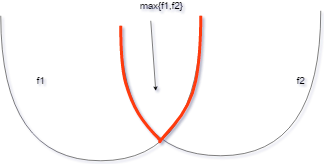
\includegraphics[]{1_3}
\item Composition with linear map.\\
$f \in cvx \R^n$, $A:\R^n \to \R^m$ is a linear map.
$f \circ A (x) = f(Ax) \in cvx \R^n$\\
\begin{align*}
f \circ A (x) & = f(A(\alpha x + (1-\alpha) y)) \\
& = f(A \alpha x + (1-\alpha) A y) \\
& \le \alpha f(Ax) + (a - \alpha) f(Ay)
\end{align*}
\end{itemize}

\end{document}